\documentclass{sigchi}

% Use this command to override the default ACM copyright statement (e.g. for preprints). 
% Consult the conference website for the camera-ready copyright statement.


%% EXAMPLE BEGIN -- HOW TO OVERRIDE THE DEFAULT COPYRIGHT STRIP -- (July 22, 2013 - Paul Baumann)
% \toappear{Permission to make digital or hard copies of all or part of this work for personal or classroom use is 	granted without fee provided that copies are not made or distributed for profit or commercial advantage and that copies bear this notice and the full citation on the first page. Copyrights for components of this work owned by others than ACM must be honored. Abstracting with credit is permitted. To copy otherwise, or republish, to post on servers or to redistribute to lists, requires prior specific permission and/or a fee. Request permissions from permissions@acm.org. \\
% {\emph{CHI'14}}, April 26--May 1, 2014, Toronto, Canada. \\
% Copyright \copyright~2014 ACM ISBN/14/04...\$15.00. \\
% DOI string from ACM form confirmation}
%% EXAMPLE END -- HOW TO OVERRIDE THE DEFAULT COPYRIGHT STRIP -- (July 22, 2013 - Paul Baumann)


% Arabic page numbers for submission. 
% Remove this line to eliminate page numbers for the camera ready copy
\pagenumbering{arabic}


% Load basic packages
\usepackage{balance}  % to better equalize the last page
\usepackage{graphics} % for EPS, load graphicx instead
\usepackage{times}    % comment if you want LaTeX's default font
\usepackage{url}      % llt: nicely formatted URLs

% llt: Define a global style for URLs, rather that the default one
\makeatletter
\def\url@leostyle{%
  \@ifundefined{selectfont}{\def\UrlFont{\sf}}{\def\UrlFont{\small\bf\ttfamily}}}
\makeatother
\urlstyle{leo}


% To make various LaTeX processors do the right thing with page size.
\def\pprw{8.5in}
\def\pprh{11in}
\special{papersize=\pprw,\pprh}
\setlength{\paperwidth}{\pprw}
\setlength{\paperheight}{\pprh}
\setlength{\pdfpagewidth}{\pprw}
\setlength{\pdfpageheight}{\pprh}

% Make sure hyperref comes last of your loaded packages, 
% to give it a fighting chance of not being over-written, 
% since its job is to redefine many LaTeX commands.
\usepackage[pdftex]{hyperref}
\hypersetup{
pdftitle={SIGCHI Conference Proceedings Format},
pdfauthor={LaTeX},
pdfkeywords={SIGCHI, proceedings, archival format},
bookmarksnumbered,
pdfstartview={FitH},
colorlinks,
citecolor=black,
filecolor=black,
linkcolor=black,
urlcolor=black,
breaklinks=true,
}

% create a shortcut to typeset table headings
\newcommand\tabhead[1]{\small\textbf{#1}}


% End of preamble. Here it comes the document.
\begin{document}

\title{Making Exchanging and Organizing Ideas Easy through Digital Affinity Diagram}

\numberofauthors{3}
\author{
  \alignauthor William Widjaja\\
    \affaddr{Department of Management of Science and technology Human-Machine interface lab, Tohoku University}\\
    \affaddr{Address}\\
    \email{william.widjaja@most.tohoku.ac.jp}\\
  \alignauthor Haruna Hayasaka \\
    \affaddr{Department of Quantum-Science Lab, Tohoku University}\\
    \affaddr{Address}\\
    \email{e-mail address}\\
    \affaddr{Optional phone number}    
  \alignauthor Masayuki Sawamura \\
    \affaddr{Affiliation}\\
    \affaddr{Address}\\
    \email{e-mail address}\\
    \affaddr{Optional phone number}
}

\maketitle

\begin{abstract}
Exchanging and organizing opinions in groups is an integral part of problem solving. One such methods commonly used is called affinity diagram. Affinity Diagramming is often created by writing individual opinions on a post-it note and collaborating with others by moving and arranging the post-it notes to form groups and links in order to makes sense of each other opinions. Despite being a common standard, this traditional paper-based methods could be improved with new technology integration. Introducing Digital Affinity Diagram system (DADS), a digital post-it note creation and organization system that integrate private creation and public organization space under one computer terminal setup. Using an extended dual-monitor to separate the two spaces, individual can build stronger personal opinions by attaching reference in private space and collaboratively organize group opinions in a cross-terminal synchronized public space.  Comparative studies are conducted to determine which of the two methods has stronger usability rating. 
\end{abstract}

\keywords{
	Guides; instructions; author's kit; conference publications;
	keywords should be separated by a semi-colon.
	\textcolor{red}{Mandatory section to be included in your final version.}
}

\category{H.5.m.}{Information Interfaces and Presentation (e.g. HCI)}{Miscellaneous}

See: \url{http://www.acm.org/about/class/1998/}
for more information and the full list of ACM classifiers
and descriptors. 
\textcolor{red}{Mandatory section to be included in your
final version. On the submission page only the classifiers'
letter-number combination will need to be entered.}

\section{Introduction}
Exchanging and organizing ideas between groups is an integral part of participatory design. One such methods commonly used to exchange and organize ideas between people is a method called affinity diagram. Affinity Diagramming is often created by writing individual ideas on a post-it note and together with other participants, they move and arrange the post-it note to create groups and links in accordance to the ideas similarities. While brainstorming is widely used as a method of idea generation, there is less work on how groups can deepen ideas.\cite{dickey2012framespaces}
 In this paper, we introduce Digital Affinity Diagram system (DADS), an individual control multi-user synchronized affinity diagram system, DADS allow each users to control the manipulation of the digital post-it note, while concurrently synchronizing the manipulation outcome across multiple users screen in real-time. The synchronization is achieved by utilizing low-latency, highly optimize network socket server which update and broadcast each manipulation command in high frequency. This technology allows allow multiple users to collaborate together in creating affinity diagram together under one single sandbox. To proof the system usefulness, we perform comparison experiment between traditional methods of affinity diagram using post-it note with DADS. Usability survey and performance metrics are calculated and analyses to determine which of the two methods is more preferred by users and determining whether DADS support users in exchanging and organizing ideas through collaborative affinity diagram. Separating public interaction space and private interaction space helps to alleviate anxiety of users. The users will have the space 
In this paper, we aim to show our developed system that aims to solve  problems that arises from  conducting exchanging of ideas through traditional methods. Based on the observation of these challenges we are able to design some technical solution to circumvent these problem and at the same time augment new capabilities to give more possibilities for users when conducting  ideas exchanging activities in group. By leveraging commonly available  and familiar technical system, we have design  an extremely user friendly  collaborative system to support and  augment the capabilities. We will perform the task and explain the problem.  task explain.  


\section{Proposed System Architecture}


\subsection{Hardware Design}


In the experiment we design a three person seating arrangement which is used, while the system can accommodate other setup such as more than 4 person and also asynchronous setup with people accessing the system from different location. However for the purpose of the experiment, We decided to setup the system in the same location using 3 seating arrangement system. 

\begin{itemize}

\item \textbf{Extended dual multi-touch monitor} - Main laptop is located at the central while the external monitor is located at the left side giving space real estate area for mouse on the right side. We choose multi-touch enabled monitor which is tilt at around 30 degree to give a sense of drawing board and also allow eye level contact for increase gaze awareness between users. 
\item \textbf{U-shape Seating arrangement} - U-shape seating arrangement is a seating design that aims to optimize the dual monitor system setup and proximity between each participants. In our experiment which we use a 3 person experiment. A common large monitor that depicts a shared  public screen , even though all the secondary screen are synchronized, the large screen serve as an assurance or affirmation that the manipulation that was perform by users actually are synced with other board. 
\item \textbf{Server setup} - Server uses windows 8 acts as a database system and the synchronized input output traffic center. Server do not require high performance for less then 5 simultaneous participants and rather than high speed performance, low latency is required to allow the high frequency setup
\end{itemize}


\begin{figure*}
\centering
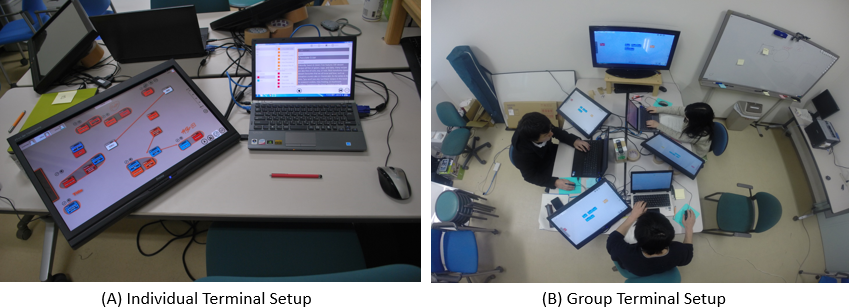
\includegraphics[width=1.9\columnwidth]{system}
\caption{{A} Single individual setup with dual extended multi touch monitor at the right side (B) 3 person group setup with a larger monitor at the center}
\label{fig:figure1}
\end{figure*}

\subsection{Software design}


The system was developed using C# using mainly .Net 4.5  framework. We build the software natively using mainly Microsoft libraries over other .net open source libraries to increase compatibility across different critical infrastructure such as server, database and clients . In addition, we also take advantage the touch framework library that is currently maturing in windows 7/8 operating system which allow us to include large screen  multi touch monitor in our  total system solution. We utilize a traditional laptop system (windows 7 powered) and extend the screen with an 22 inc iiyama multitouch monitor. The multitouch monitor uses four point infrared sensor to detect accurate multitouch from users and has a response time of 8 ms.
We chose a dual-screen design to increase information display clarity and focus for the users. While the main Private input screen will act as each user's personal input interface,  the public board will focus on collaboration. 


\subsubsection{Private Space Interface}
The interface  is designed so to maximize visibility and navigation capabilities for users to view both own points and other points. There is 5 area of design in the private dashboard The private space interface is a interface dashboard that is used for users to input all the opinions and ideas, in fig 1, there is 3 column dashboard in the top right hand is the selection between different topic which allows users to switch from one topic to another, while next to it in the middle column dashboard is the listing of all the opinion titles written by the individuals, bottom right corner is where users select and view different participants points and next in the middle bottom column is where listing of other participants points title. Finally the full screen right column is where users input own points. Users can switch freely between the input dashboard and a browser window when they are searching for supporting material.
\begin{figure}
\centering
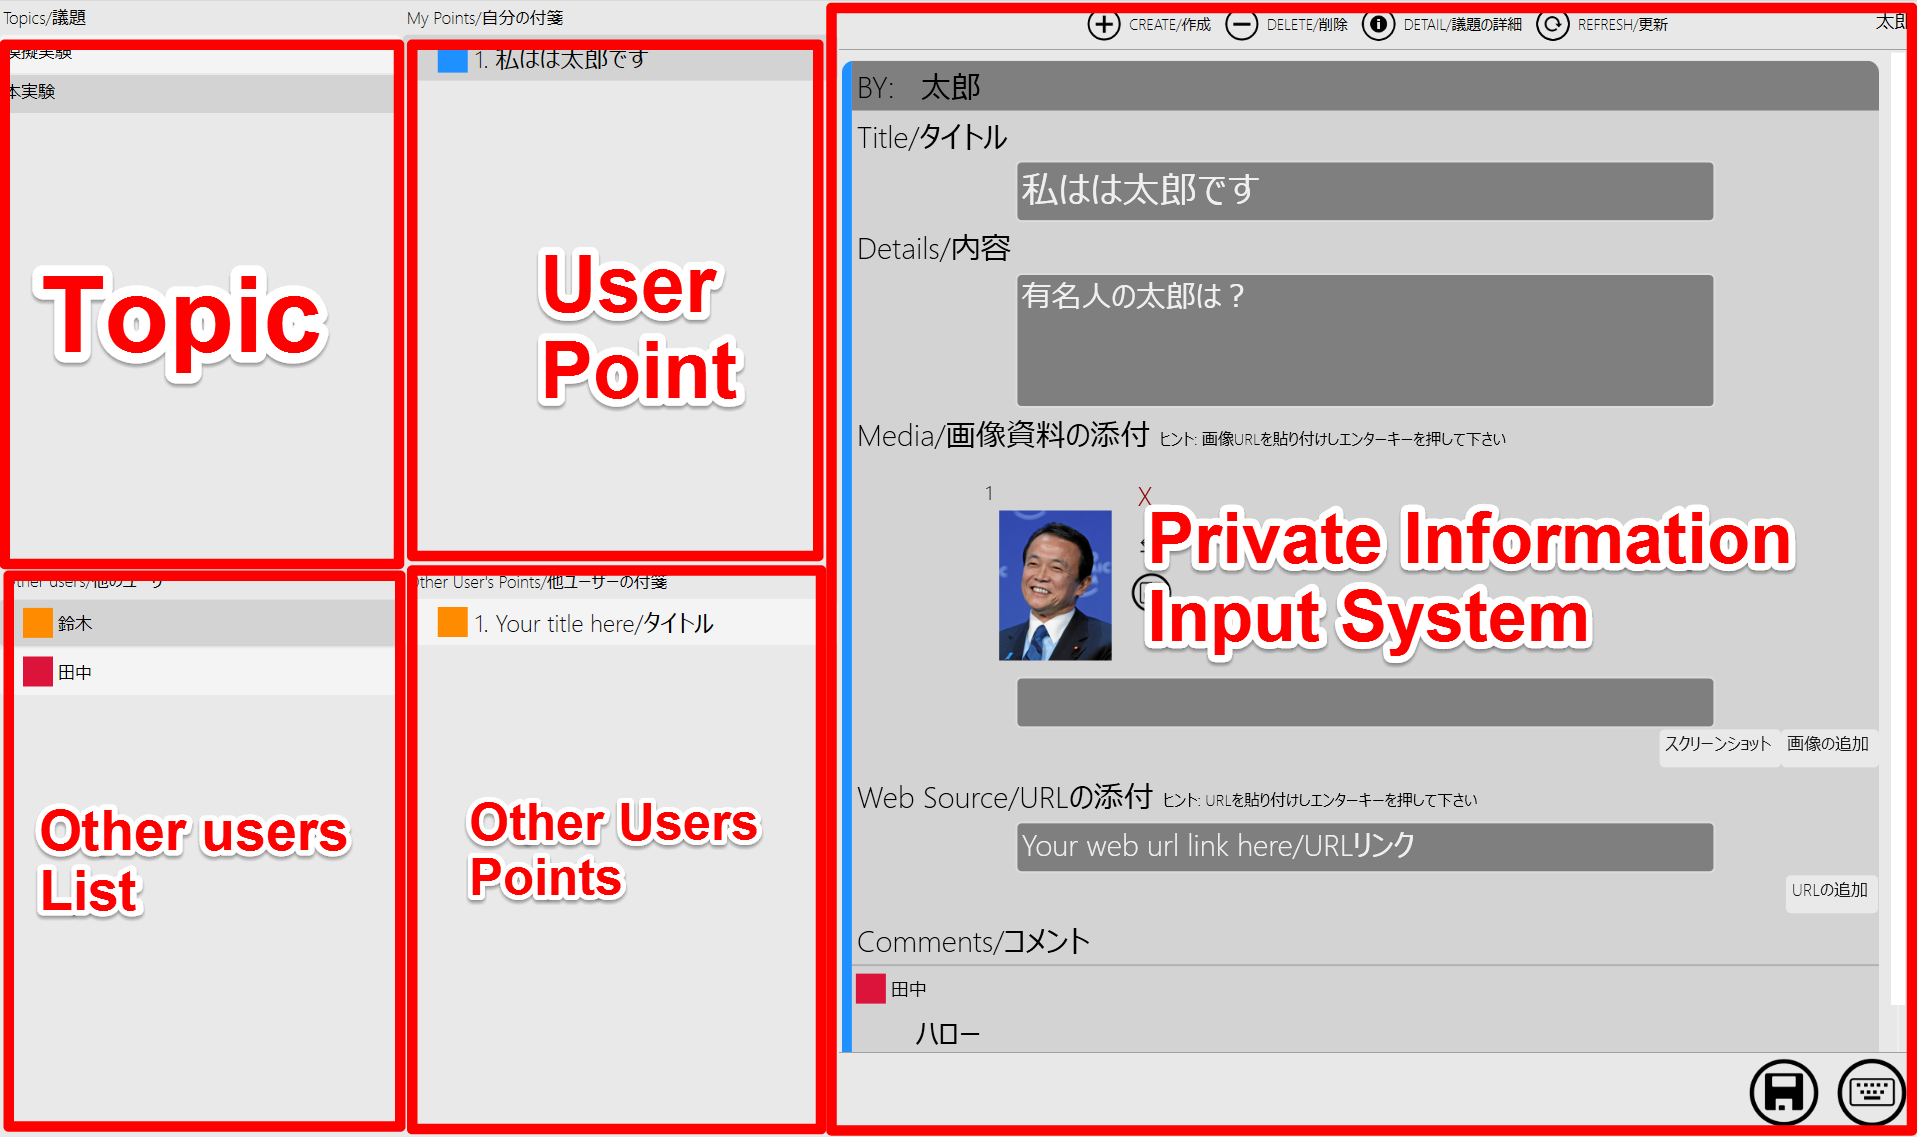
\includegraphics[width=1.0\columnwidth]{private}
\caption{Private Space User Interface}
\label{fig:figure1}
\end{figure}

\begin{itemize}


\item Discussion Room - Like all gaming technology, each discussion  topic are treated as a room.  Users will have to write their name and select the pre-determine color they wish to have. Once selecting their identity, they will choose the discussion room they intend to participate and upon entering each users have their own color identity to present them 
\item  Input and Navigating-To optimize the ease of navigation and ease of inputting text, 3 column design interface are used. The first column is divided between topic selection on the top and bottom is the users election while in the top second column show individual idea points and bottom second column show others idea points . The third column will have the most space for inputting the ideas
\item Idea input - Input form are divided into 3 input  areas, First input is the title of their ideas, Second is the description of their ideas and  the third input is the source  attached to support their ideas
\item Attachment System - We observed early on the development phase  that users often search more information about their ideas and on the Internet and uses sources to verify or affirm  their ideas. To support this behavior, we create a source attachment function to give users ability to quickly attach article or media sources from the Internet to their ideas. 
\begin{itemize}
  \item  Media Attachment - We choose the familiar copy and paste functions to upload images from the web, while browsing on the Internet browser users are able to right click the images they wish to upload and copy and paste the image url to our media text box in the system private input form, The code will automatically detect the presence of the media and its traditional format ( jpg, bmp) . If the url link is not in the right format an error message will be shown, but if the media is detected with the right image format,  thumbnail of the attached images will be shown.

  \item Screen shot - Another function is screen shot function, We observe that in some website users would like to capture an areas of the website (images plus text ) or graph that is not compatible with the standard image format ( video screen shot) , thus using the screen shot function. After pressing the screen shot function in the system, the screen will be brought to the main web browser where users can scroll up and down the desired screen. click next will initiate the screen shot capture where users need to drag from top left to bottom right the desired area of the screen they wish to capture, once letting go the drag. Automatically the screen shot thumbnail will be displayed at the private input screen. this indicated that screenshot capture is successful. 
\end{itemize}

The private space interface allows users to easily create points related to a topic and populate them with information using familiar cut-and-paste mechanics. A basic interaction process would involve selecting the topic from the Topic window (pictured in Figure 1) and creating a new point in the User Point window, which creates a new card on the Public Information space related to that topic. Users can be identified as the author of a point by the color of the card. After creating a point, users can illustrate their point by adding supplementary information, images, and links in the Private Information Input window. When they are done adding information, the card is complete and they can create a new point, or browse other users' points, just as in the analog version of AD creation.

\subsubsection{Public Space Interaction}

\begin{figure}[!h]
\centering
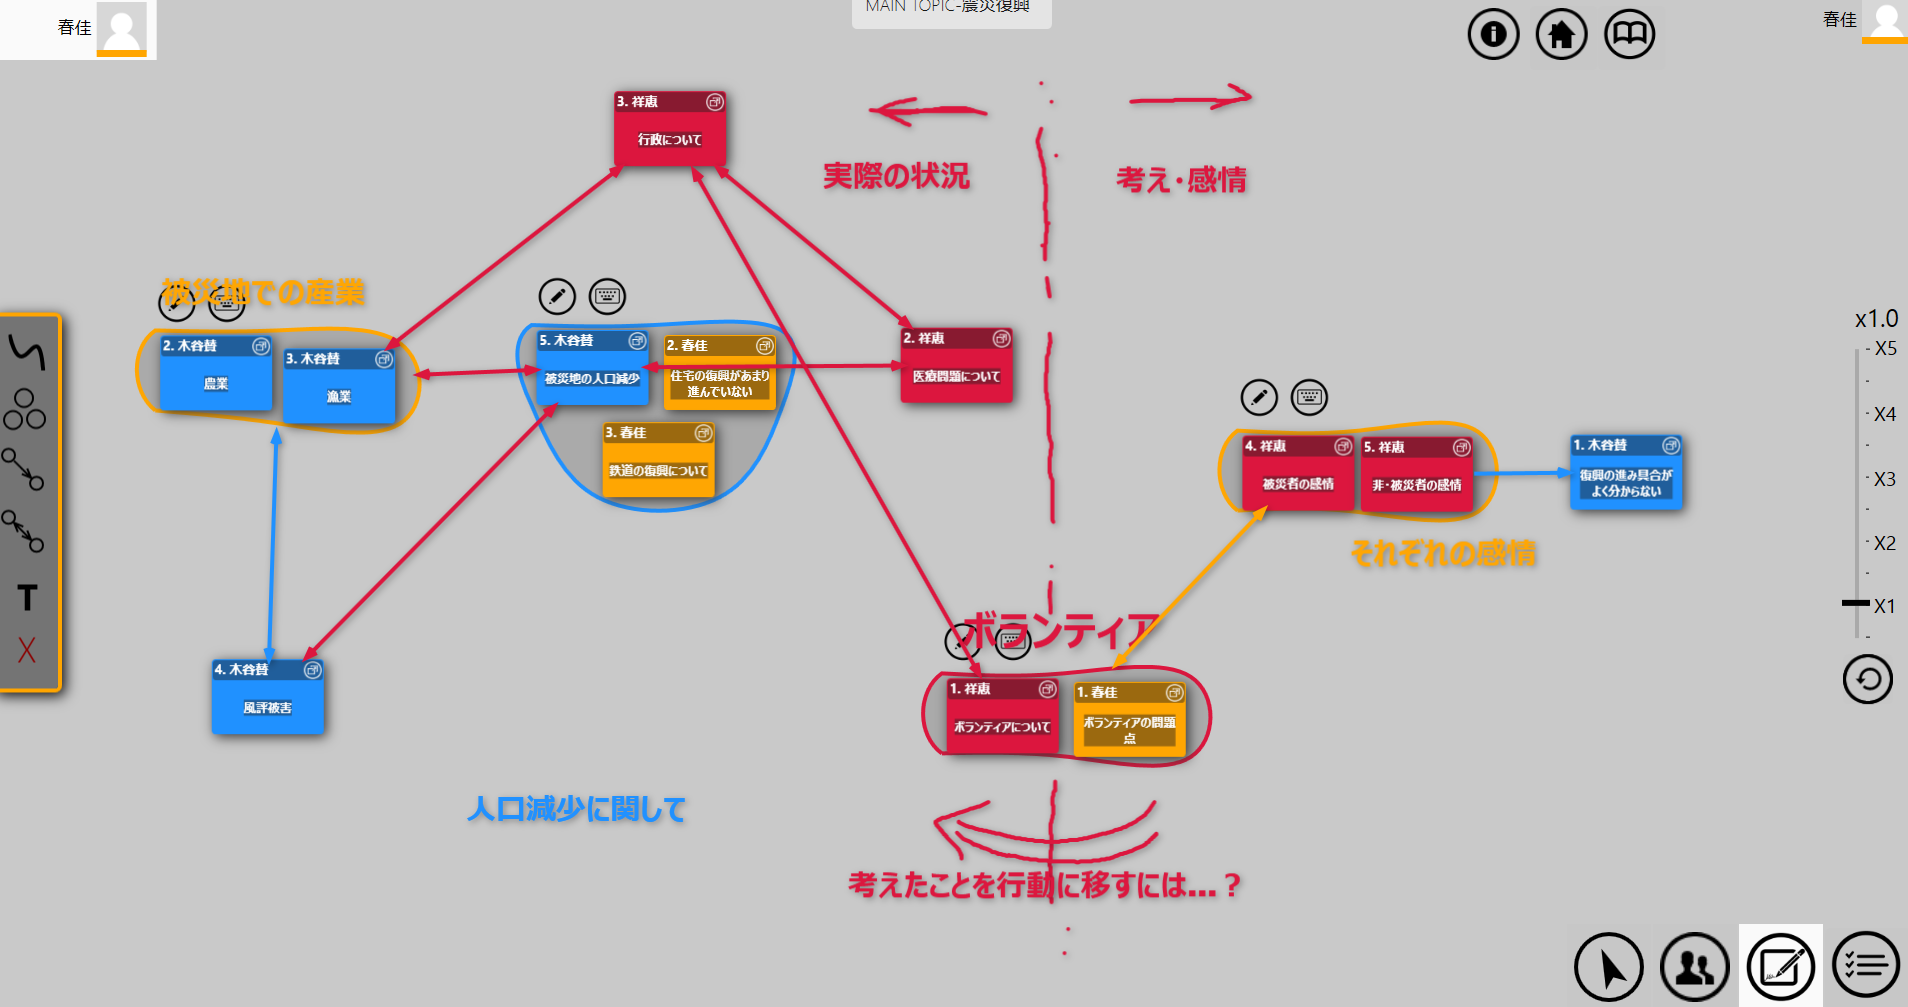
\includegraphics[width=1.0\columnwidth]{public1}
\caption{Screenshot of Public Interface.}
\label{fig:figure1}
\end{figure}
In the public space interaction, points that are written on the private space are displayed in public space in a form of card with the users identity color, the card is filled with title of the points and name, these card can be moved multi-directional to be rearrange by the users.

In our observation, we strongly hypothesize that to achieve collaboration, the public board has to be synchronized smoothly across different users. To achieve the goal, we utilize the core technology from the massive multi player gaming (MMOG) system which uses network socket and adapt the technology to suit our system. Participants which uses our system are treated like players in the MMOG system where we give each participants an identity and manipulation capabilities such as idea boxes movement and details enlargement. These manipulation input command are constantly sent to the server ( Up to 15 input command per second )  to the server and broadcast ( Up to 15 output command per second ) to other clients to update.  The low latency will determine the smoothness of the control and manipulation response. 


In addition there are about 4 main features in the public space that allows users to conduct affinity diagram  that can allow the users to do in the public dashboard they are 

\begin{itemize}


\item  \textbf{In-depth Details Card expansion}   - All the cards displayed only the title of the users points, there is a function to expand the card details by double clicking on the card, This will trigger a windows that display all of the in-depth details of the card include the description, attached links and sources. 
\item  \textbf{Presentation Mode} -The card expansion function are individual controlled, whenever it is appropriate, users can synchronized the card expansion function with other clients, this function is an aid to help users control and present their points easily, the synchronized card expansion help users to use the expansion of the card 
\item \textbf{Grouping and Linking} -  Grouping and linking is a function where users are can group using a circular motion, if the users initiate the group button and initiate a circular motion between numerous card , a circular line is displayed to show the grouped card and these grouped card can be move in various direction, another important part is the reorganize the group function, users can move any card within the group and using 2 corner touch algorithm where if any 2 corner of the card touch the group it will initiate  a regroup function that allow users to insert a new card into the group and vice versa. linking is also done when users initiate the link function and click the two card in sequence  
\item \textbf{Vector Free Draw system} - The free Draw System is a function where, we users can freely on the public space unlike typical drawing system, we used a new methods called vectored drawing, where the draw divided into vectored, Each time users draw, users need to initate a finish draw function where the draw are converted to object vector , where users can move resize the draw, this is designed to give flexibility for the users to organize the draw around 
\item \textbf{Commenting System} - This new function is allowing users to comment on each other points to ask question and write  thoughts on the system, users can expand the card and write comments on others person points . In addition, notification algorithm are created to notify users of a new comment coming in , this allow users to have a real-time exchanges of comment with each other. 



\subsection{Testing the system}
We identify four main area of activities  that is commonly used  in typical group work for exchanging ideas. The four common activities are also designed to be linear and in order. 

\begin{enumerate}
\item Idea Creation -Idea creation is an activities where users create a new ideas based on his or her perception on a single topic. If given internet access, there are two common behavior during the idea creation phase. One is start  writing immediately and search the internet to verify their ideas and another behavior is the search for idea inspiration on the internet and write the ideas based on their surfing. Nevertheless, both behavior benefited by attaching the internet sources ( images or url link ) to their ideas. 
\item Presenting - Despite the ideas are shown visible by other users, It is more convincing that the idea is explain by the creator, thus our goal is to build a system that needs to make the users explain their points easily. Using common sense, that the availability of a source to support the ideas will increase the confidence of each users. Thus creating a system that allows users to control and broadcast their sources during explanation phase will definitely increase ease of explanation and increase understanding level of others. 
\item Commenting and Exchange Ideas -Each ideas are unique in nature and questions and critics are asked regarding points. Thus we think that it is important that users can easily navigate to specific points and leave a comment. We also noticed that it is important that users are notified when there is a new comment written on their points. so users are able to response to the comments written by other users. 
\item Collaborative Affinity Diagram -To organize all the users ideas to give a common overview of the opinions of the group, we utilize the methods called affinity diagram to organize the ideas. Affinity diagram is a simple methods that groups and link similar and related points and ideas to give a better clarity to the simplicity of the overall group ideas. The clarity of the group ideas is the precursor for any problem solving tasks and having strong common overview will help participation design activities such as solving problem or creating solution more effectively. 
\end{enumerate}

\subsection{Methodologies}

We setup two type of idea exchange environment named as Analog methods and Digital methods. In analog methods traditional tools are used including white board, colored sticky note and colored marker. Ideas and comments are written on a numbered  sticky note. Users will need to write their ideas title using bold marker and comment are written using black pen. The comments  are pasted below the ideas the users wish to comment which also act as a connection to the ideas and comments. To make the experiment equally balance, we allow users to search the Internet and print any sources in paper. Users also are required to write numbers on the printed article papers according the the numbered sticky note. Magnets are provided to sticky the printed articles on the white-board. In Digital environment, the system are used to conduct the experiment tasks. Before the experiment participants are given instruction and the tutorials on how to use the system. Upon completing the experiment subjects are invited to participate in a survey to compare and evaluate the usability of the system between analog and digital using a rating scale.

\begin{figure}[!h]
\centering
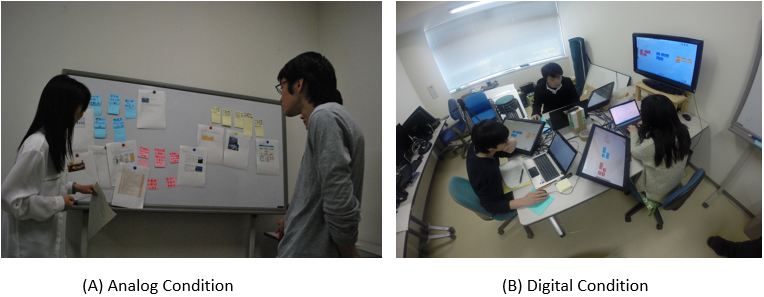
\includegraphics[width=1.0\columnwidth]{condition}
\caption{(A) Experimental Condition in Analog Condition using sticky note and white board (B) Experimental condition in Digital condition using DADS.}
\label{fig:figure1}
\end{figure}


\subsection{Experiment Procedure}

To prove that our system helps users to perform basic tasks in idea exchanging activities easier, we have conducted a comparison studies between traditional methods of idea exchanging  with our system. We choose a 3 person experiment which depicts the odd number to prevent group forming within the experiment. ( If there is 4-person, there is a possibility that 2 person groups are formed ). We divide the experiment in 4 commonly perform tasks in a typical idea exchange activities and measure the usability.  We give users a two equally popular topic in our host university as the topics of discussion. We also divide the experiment into 4 task

Participants were welcomed and introduced to the purpose of the study. They were then given brief instructions on using the Digital Affinity Diagram System for about 30 minutes, and another 30 minutes to try out the system in the tutorial mock up scenario to become familiar with the systems and discover system functionality. The experiment schedule and task was then explained to the group before starting the experiment. 

\begin{itemize}
\item \textbf{Task 1- 5 ideas and attach sources} - Each users are given 30 minutes to create 5 ideas on the topic. They are allowed freedom of access to the internet to search attach their ideas. 
\item \textbf{Task 2 - Present  ideas to others } - Each users are given time to present and explain their points to the rest of the participants. 
\item \textbf{Task 3 - Exchanging comment with each other} - The group is given 20 minutes to comment on others points and at the same time reply any comment posted to them. They are asked to write as much comment as possible across all the ideas until the time is up. 

\item \textbf{Task 4- Affinity Diagram} - After completing the comment exchange task, they are then ask to collaborate to create an affinity diagram using the ideas created earlier, they are asked to group similar ideas and also link related ideas. 
\end{itemize}
All experiment subject need to complete all 4 tasks in both analog and digital methods (Total=8 tasks) in each experiment group. The order of methods are also evenly rotated in each group which means that when one experiment group start with analog then continue with digital, the next experiment will start with digital and continue with analog, this is required to balance the data. Total experiments with rest took around 5 1/2 hours to complete. 

\subsection{Observation}

\begin{table*}[ht]
\centering
\caption {Result of the Survey metrics}
\begin{tabular}{rrrrrrrrrrr}
  \hline
 & N & Mean & SD & SE & 95\%LCI & 95\%UCI & Median & Skewness & Kurtosis & P-Value \\ 
  \hline
  
Create Points AN & 12.00 & 3.17 & 1.11 & 0.32 & 2.46 & 3.87 & 3.00 & 0.07 & -0.46 & 0.04 \\ 
  Create Points DI & 12.00 & 4.17 & 1.03 & 0.30 & 3.51 & 4.82 & 4.50 & -0.75 & -0.88 &  \\ 
    \hline
  Edit Points AN & 12.00 & 2.58 & 0.90 & 0.26 & 2.01 & 3.16 & 2.50 & 0.12 & -1.09 & 0.00 \\ 
  Edit Points DI & 12.00 & 4.17 & 1.34 & 0.39 & 3.32 & 5.02 & 5.00 & -1.32 & 0.28 &  \\ 
    \hline
  Attach Source AN & 12.00 & 2.00 & 0.85 & 0.25 & 1.46 & 2.54 & 2.00 & 0.00 & -1.74 & 0.00 \\ 
  Attach Source DI & 12.00 & 4.58 & 0.67 & 0.19 & 4.16 & 5.01 & 5.00 & -1.11 & -0.13 &  \\ 
    \hline
  Show Points AN & 12.00 & 2.25 & 0.97 & 0.28 & 1.64 & 2.86 & 2.00 & 0.10 & -1.27 & 0.00 \\ 
  Show Points DI & 12.00 & 4.25 & 0.97 & 0.28 & 3.64 & 4.86 & 4.50 & -1.01 & -0.12 &  \\ 
  \hline
  Explain Points AN & 12.00 & 3.50 & 0.67 & 0.19 & 3.07 & 3.93 & 3.00 & 0.82 & -0.68 & 0.46 \\ 
  Explain Points DI & 12.00 & 3.75 & 1.06 & 0.30 & 3.08 & 4.42 & 4.00 & -0.40 & -1.20 &  \\ 
  \hline
  Navigate Points AN & 12.00 & 2.50 & 1.00 & 0.29 & 1.86 & 3.14 & 2.00 & 1.00 & 0.73 & 0.00 \\ 
  Navigate Points DI & 12.00 & 4.33 & 0.65 & 0.19 & 3.92 & 4.75 & 4.00 & -0.34 & -1.05 &  \\ 
  \hline
  Understand Points AN & 12.00 & 3.25 & 0.97 & 0.28 & 2.64 & 3.86 & 3.00 & 0.66 & -0.70 & 0.04 \\ 
  Understand Points DI & 12.00 & 4.00 & 0.85 & 0.25 & 3.46 & 4.54 & 4.00 & -0.81 & 0.15 &  \\ 
  \hline
  Read Comments AN & 12.00 & 2.67 & 1.23 & 0.36 & 1.88 & 3.45 & 2.00 & 0.85 & -0.52 & 0.00 \\ 
  Read Comments  DI & 12.00 & 4.50 & 0.67 & 0.19 & 4.07 & 4.93 & 5.00 & -0.82 & -0.68 &  \\ 
  \hline
  Write Comments AN & 12.00 & 2.33 & 0.98 & 0.28 & 1.71 & 2.96 & 2.00 & 0.43 & -1.03 & 0.00 \\ 
  Write Comments  DI & 12.00 & 4.50 & 0.67 & 0.19 & 4.07 & 4.93 & 5.00 & -0.82 & -0.68 &  \\ 
  \hline
  Reply Comments AN & 12.00 & 2.33 & 1.15 & 0.33 & 1.60 & 3.07 & 2.00 & 0.70 & -0.15 & 0.00 \\ 
  Reply Comments  DI & 12.00 & 4.33 & 0.89 & 0.26 & 3.77 & 4.90 & 4.50 & -1.32 & 1.15 &  \\ 
  \hline
  Create Affinity Diagram AN & 12.00 & 2.58 & 1.00 & 0.29 & 1.95 & 3.22 & 3.00 & -0.21 & -1.21 & 0.01 \\ 
  Create Affinity Diagram DI & 12.00 & 4.00 & 0.74 & 0.21 & 3.53 & 4.47 & 4.00 & 0.00 & -1.32 &  \\ 
 \hline
  Teamwork AN & 12.00 & 3.25 & 1.29 & 0.37 & 2.43 & 4.07 & 3.00 & -0.42 & -0.85 & 0.70 \\ 
  Teamwork DI & 12.00 & 3.42 & 1.16 & 0.34 & 2.68 & 4.16 & 3.50 & -0.45 & -0.68 &  \\ 
   \hline
  Comfort AN & 12.00 & 3.25 & 1.22 & 0.35 & 2.48 & 4.02 & 3.00 & -0.16 & -1.08 & 0.04 \\ 
  Comfort DI & 12.00 & 3.92 & 0.79 & 0.23 & 3.41 & 4.42 & 4.00 & -0.88 & 0.57 &  \\ 
   \hline
  Usefulness AN & 12.00 & 3.33 & 1.15 & 0.33 & 2.60 & 4.07 & 4.00 & -0.60 & -0.90 & 0.02 \\ 
  Usefulness DI & 12.00 & 4.42 & 0.67 & 0.19 & 3.99 & 4.84 & 4.50 & -0.56 & -0.97 &  \\ 
   \hline
  Satisfaction AN & 12.00 & 3.00 & 1.21 & 0.35 & 2.23 & 3.77 & 3.00 & 0.29 & -0.95 & 0.02 \\ 
  Satisfaction DI & 12.00 & 4.08 & 0.79 & 0.23 & 3.58 & 4.59 & 4.00 & -0.12 & -1.53 &  \\ 
   \hline
\end{tabular}
\end{table*}


 Twelve  participants from the university  were asked to test the DADS System discussion room. All participants were divided into groups of 3. There were 7 females and 5 males between the age of 18 and 24.  Participants spent an average of 5.9 (SD=3.4) hours a day on a computer a. Participants reported having an average of 2.8 meetings per week (SD=3.45), 


\section{Measurement}
In this experiment we tried to measure the usability of the system in making them create points. 
Those who participate on the experiment  took a rating scale questionnaire to evaluate the ease of completing the task based on two methods. The rating scale ranges  from 1 being most negative and 5 being most positive.  Based on the self rating survey Users must evaluate their perception on both analog and digital and give the score on the following 9 questions . 

\begin{enumerate}
  \item Ease of Point Creation- This question is asked on whether how easy is the users feel when creating any new points 
  \item Editing Points - This question asked about how easy is it for users when editing the content of the points 
  \item Attaching Source - This question compared the  usability by users in using attached sources in digital compared using printing sources 
  \item Navigating Points - This question is about navigating between own points and other points. 
  \item Showing Source - This question is about how easy is it to show points ans resources to other users 
  \item Writing Comments - This question ask about how easy is it to write comments 
  \item Replying Comments -This question ask about how easy is it to reply  comments 
  \item Creating Affinity Diagram - This question ask about how flexible is it to create affinity diagram 
  \item Usefulness -This question ask to compare the level of usefulness compared to the two methods  
  \item Satisfaction of Result - This question ask about how satisfied are the users in regards to the final affinity diagram result   
\end{enumerate}



\section{Observation}





\section{Conclusion}

In this experiment, we have discovered that the developed system has extremely high usability rating from the users, Action task such as creating, navigating the ideas is more preferred  in digital compared to analog, In addition, the number of attachment of sources proves to be higher in digital system with the copy and paste system compared to the print system. Commenting each other points on text based methods is also easier in the digital compared to analog with consistent result, that writing, reading and replying comments is easier in digital compared to analog.  However, when we probe the question whether the system helps them to better understand the content of other people users, We found no significant difference between analog and digital system. In addition, we also ask the question the level of teamwork, we also find no significant difference between the two methods. This means that the digital system can maintain the same level of teamwork in digital despite having  them working from different platform. Moreover, We also conclude that group spend spend more time in creating affinity diagram and perform an average  7 30 mins more in digital compared in analog. We believed the extra time is not factored because of difficulty of coordinating the affinity diagram, We believed that it is because, the ease of the system allows them to be more flexible in their activities which show that  movement of ideaboxes in digital is 4 times more than analog. which leads them to do affinity diagram much deeper. Finally users also conclude that it they have a higher level of satisfaction on the digital made content compared to the analog made content which conclude that based on this experiment that  digital methods do create a better perceived satisfaction of ideas organization compared to traditional analog methods. This proves many of various benefit of the system in helping users to exchange and organize ideas better. 


\section{Acknowledgments}

We thank CHI, PDC and CSCW volunteers, and all publications support
and staff, who wrote and provided helpful comments on previous
versions of this document.  Some of the references cited in this paper
are included for illustrative purposes only.  \textbf{Don't forget
to acknowledge funding sources as well}, so you don't wind up
having to correct it later.

% Balancing columns in a ref list is a bit of a pain because you
% either use a hack like flushend or balance, or manually insert
% a column break.  http://www.tex.ac.uk/cgi-bin/texfaq2html?label=balance
% multicols doesn't work because we're already in two-column mode,
% and flushend isn't awesome, so I choose balance.  See this
% for more info: http://cs.brown.edu/system/software/latex/doc/balance.pdf
%
% Note that in a perfect world balance wants to be in the first
% column of the last page.
%
% If balance doesn't work for you, you can remove that and
% hard-code a column break into the bbl file right before you
% submit:
%
% http://stackoverflow.com/questions/2149854/how-to-manually-equalize-columns-
% in-an-ieee-paper-if-using-bibtex
%
% Or, just remove \balance and give up on balancing the last page.
%
\balance

\section{References format}
References must be the same font size as other body text.
% REFERENCES FORMAT
% References must be the same font size as other body text.

\bibliographystyle{acm-sigchi}
\bibliography{sample}
\end{document}
